\documentclass{article}
\usepackage{graphicx} % Required for inserting images
\usepackage{tcolorbox}
\usepackage{amsmath}
\usepackage{ulem}


\title{Module 2}
\author{Sid S}
\date{September 2023}

\begin{document}

\section*{Set Operations}
SQL alternates between using \textit{bags} and \textit{sets} to contain query results. Recall that sets contain no duplicate elements whereas a bag, or multiset, may contain multiple copies of the same element. So every set is a bag, but not every bag is a set. Notice how the query below outputs a bag since the output can include duplicate values:

\begin{tcolorbox}
    \begin{verbatim}
        SELECT R.A
        FROM R, S, T
        WHERE R.A = S.A OR R.A = T.A;
    \end{verbatim}
\end{tcolorbox}

Use of the \textit{DISTINCT} keyword can cause this output to become a set:

\begin{tcolorbox}
    \begin{verbatim}
        SELECT DISTINCT R.A
        FROM R, S, T
        WHERE R.A = S.A OR R.A = T.A;
    \end{verbatim}
\end{tcolorbox}

Set operations, on the other hand, default to set semantics rather than bag semantics. 

Set operations generally take this format:

\begin{tcolorbox}
    \begin{verbatim}
        (SELECT ... FROM ... WHERE ...)
        {op}
        (SELECT ... FROM ... WHERE ...);
    \end{verbatim}
    where \textit{\{op\}} is one of:
    \begin{itemize}
        \item \textit{UNION}
        \item \textit{INTERSECT}
        \item \textit{MINUS/EXCEPT}
    \end{itemize}
\end{tcolorbox}

Importantly, the relations we are conducting set operations on must share the same schema, aka they must be union-compatible. Furthermore, we may switch to bag semantics by using the keyword \textit{ALL}. And recall that \textit{UNION} refers to all distinct elements from either relation, \textit{INTERSECT} refers to all distinct elements that overlap between the two relations, and \textit{MINUS/EXCEPT} refers to all distinct elements that are in one relation with all elements overlapping with the other relation removed. Just keep in mind that many DBs do not support the final two operations.

Also keep in mind that the two component relations in a set operation may not share all of the same attributes to meet the requirement of sharing the same schema. Rather, the query output for each relation must output a relation with a schema that matches that of the other. And this doesn't require attribute names to match either, just the data types should be the same. For instance, let's try some queries on the following relations:

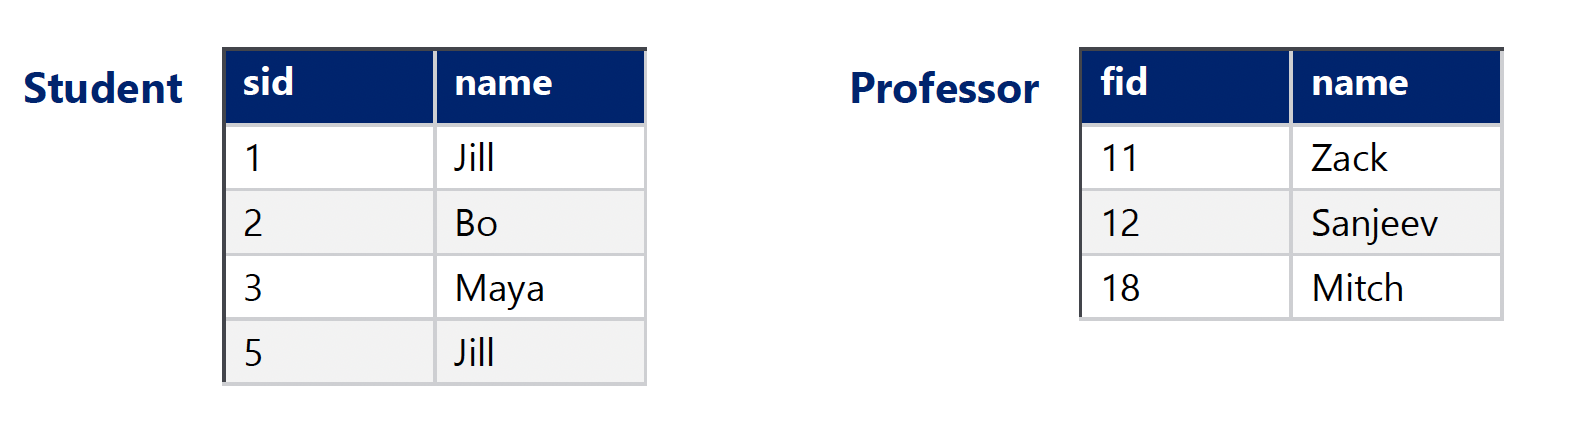
\includegraphics[width=10cm]{Assets/studentProfExample.png}

Let's print the names of all people from the above relations:

\begin{tcolorbox}
    \begin{verbatim}
        (SELECT name
        FROM Student)
        UNION
        (SELECT name
        FROM Professor);
    \end{verbatim}
\end{tcolorbox}

Recall that set operations default to outputting sets, so only distinct elements. We can, however, modify the query to include duplicates:

\begin{tcolorbox}
    \begin{verbatim}
        (SELECT name
        FROM Student)
        UNION ALL
        (SELECT name
        FROM Professor);
    \end{verbatim}
\end{tcolorbox}

What if we want to print the ids of students who are not taking a course, looking at the below relations -- using the \textit{MINUS} keyword?

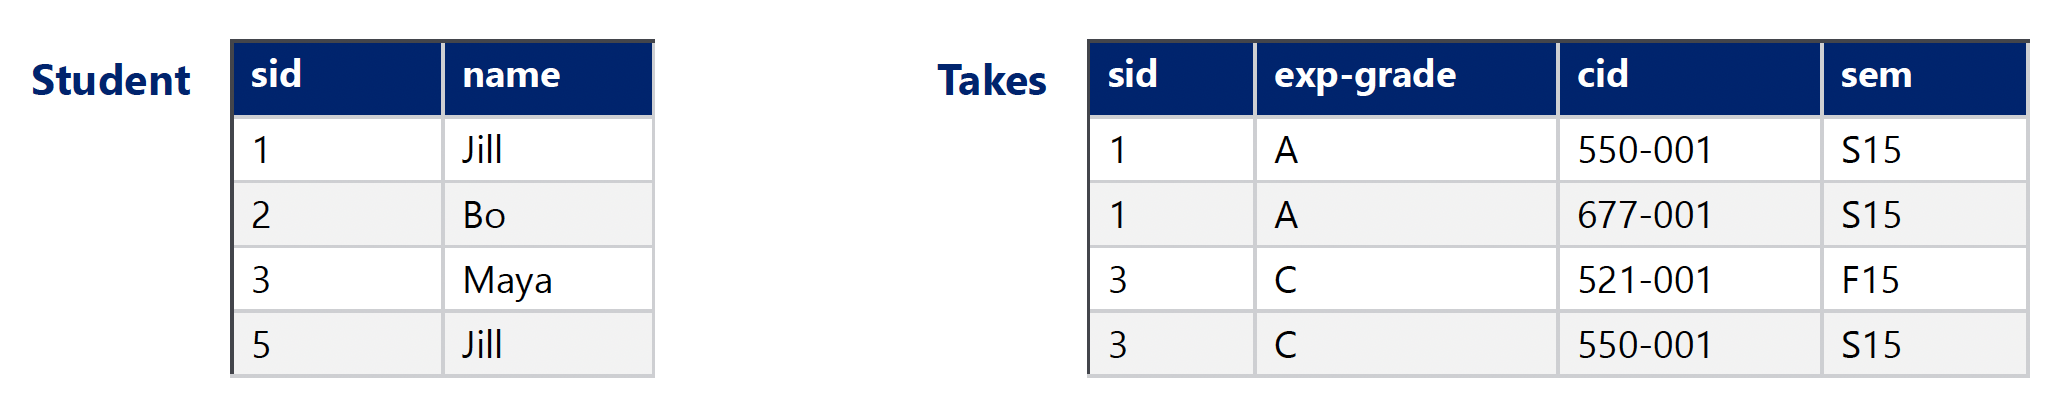
\includegraphics[width=10cm]{Assets/studentClassExample.png}

\begin{tcolorbox}
    \begin{verbatim}
        (SELECT sid
        FROM Student)
        MINUS
        (SELECT sid
        FROM Takes);
    \end{verbatim}
\end{tcolorbox}

What if we want to print the ids of students who are taking some course -- using the keyword \textit{INTERSECT}?

\begin{tcolorbox}
    \begin{verbatim}
        (SELECT sid
        FROM Student)
        INTERSECT
        (SELECT sid
        FROM Takes);
    \end{verbatim}
\end{tcolorbox}

We could have also accomplished the same thing as above using the \textit{JOIN...ON} syntax. 

\begin{tcolorbox}
    \begin{verbatim}
        SELECT DISTINCT s.sid
        FROM Student s JOIN Takes t
            ON s.sid = t.sid;
    \end{verbatim}
\end{tcolorbox}

And this is just basic logic, but keep in mind that \textit{INTERSECT} can be expressed using \textit{MINUS}. Visualize a venn diagram and it should become apparent that given two overlapping relations \textit{R} and \textit{S}, $R \cap S = R - (R - S)$

\section*{Subqueries: \textit{IN}/\textit{NOT IN}, \textit{ALL}/\textit{ANY}}

A subquery can occur in the \textit{WHERE} clause of a query. An \textbf{uncorrelated} subquery occurs independently of the outer query whereas a \textbf{correlated} subquery refers to variables in the outer query. 

Let's first take a look at an uncorrelated subquery:

\begin{tcolorbox}
    \begin{verbatim}
        SELECT sid
        FROM Takes
        WHERE cid IN
            (SELECT cid
                FROM Takes
                WHERE sid=1)
    \end{verbatim}
\end{tcolorbox}

Now, let's take a look at a correlated subquery:

\begin{tcolorbox}
    \begin{verbatim}
        SELECT sid, name
        FROM Student s
        WHERE EXISTS
            (SELECT t.sid
                FROM Takes t
                WHERE s.sid = t.sid)
    \end{verbatim}
\end{tcolorbox}
Notice how the correlated subquery referred to the relation alias \textit{s} from the outer query.

Now, let us try to understand what the \textit{IN} and \textit{NOT IN} syntax mean. First of all, both of them have this particular format:

\begin{tcolorbox}
    \begin{verbatim}
        {attr} IN {subquery}
        {attr} NOT IN {subquery}
    \end{verbatim}
\end{tcolorbox}

These syntax basically test for membership/non-membership of an attribute in the subquery result. Alright, now let's use some relations to work through examples with these syntax:

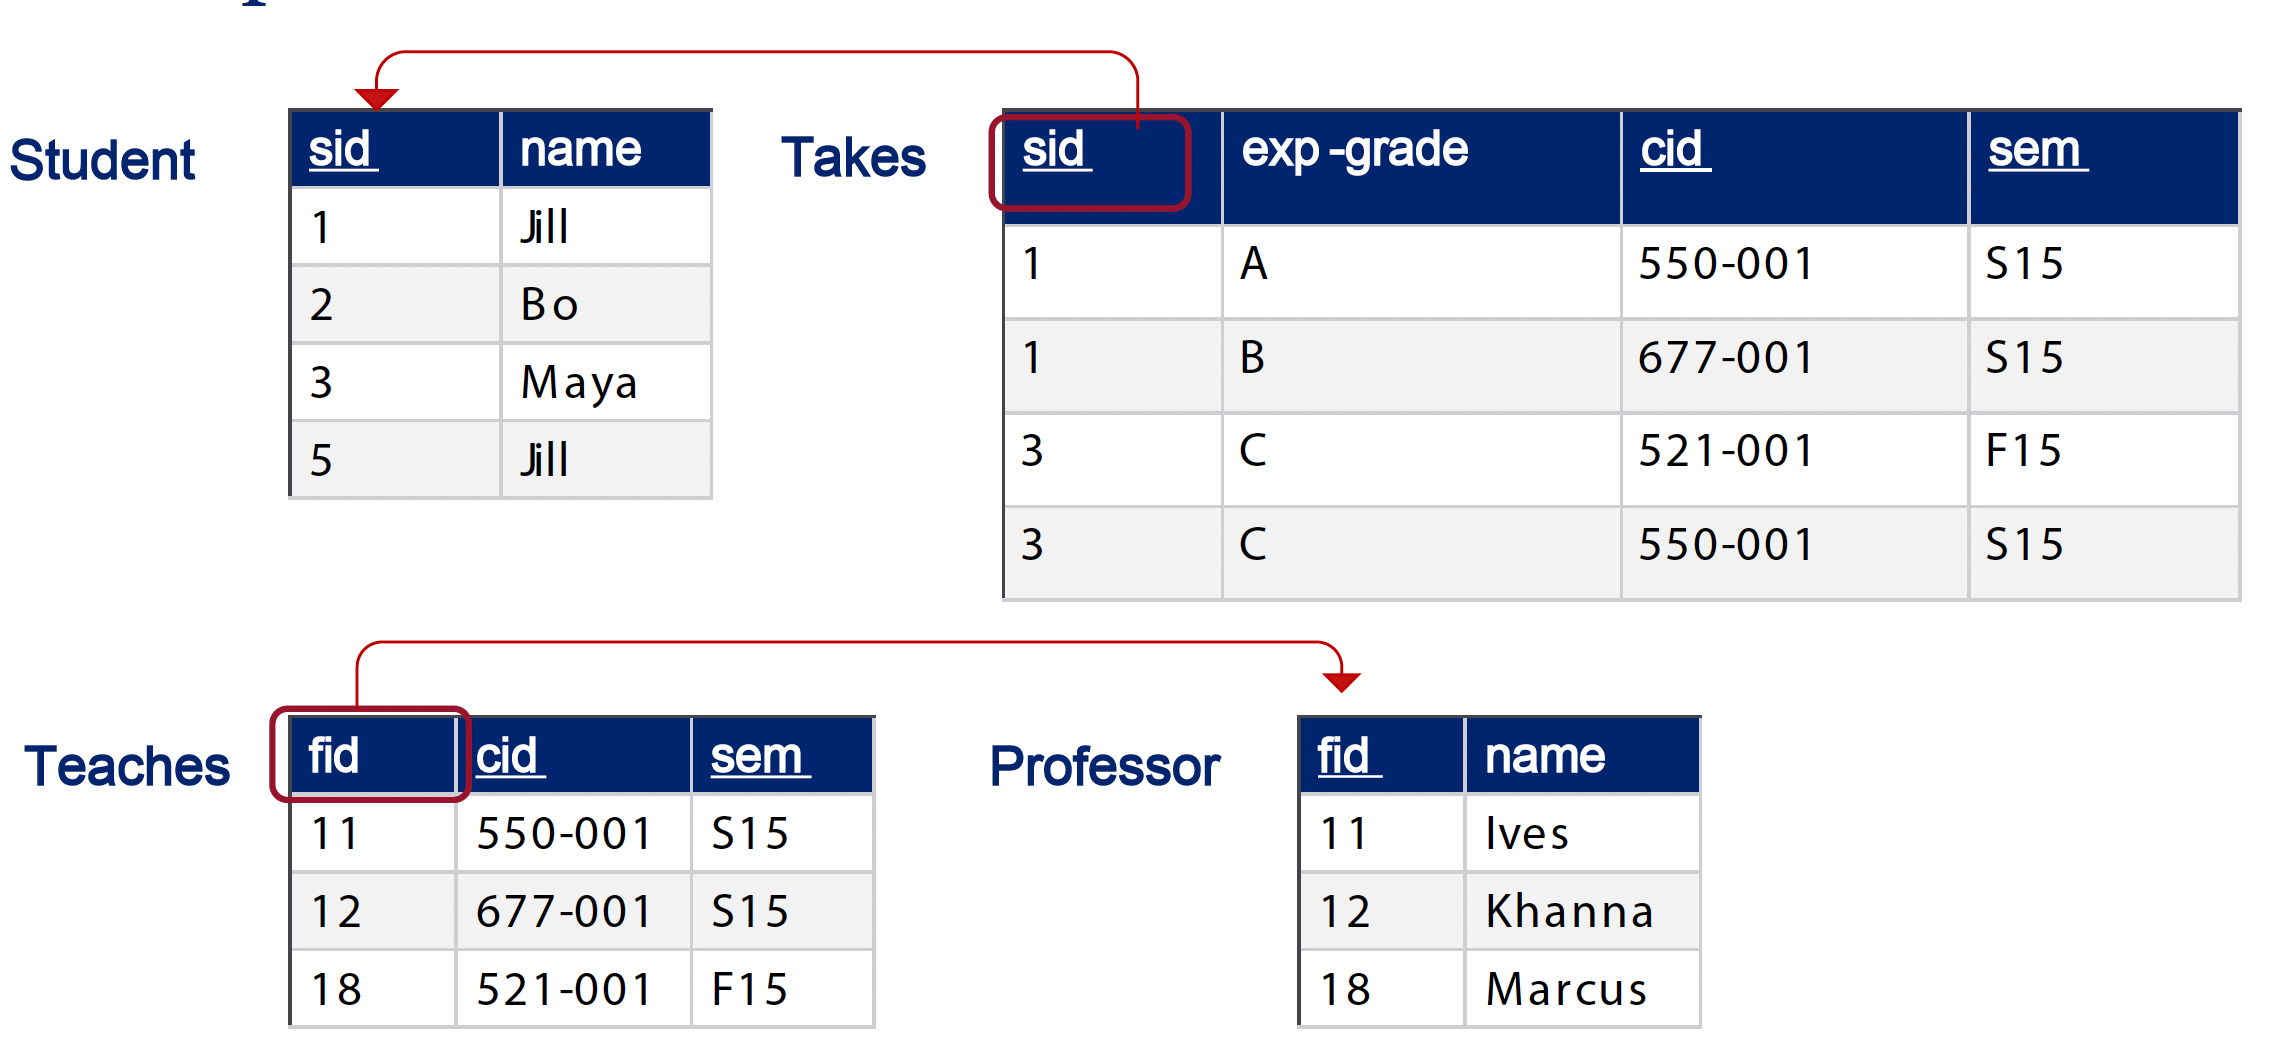
\includegraphics[width=10cm]{Assets/subqueriesExample.png}

Now, let us use the \textit{IN} syntax to get all students who have taken a course by Prof. Marcus.

\begin{tcolorbox}
    \begin{verbatim}
        SELECT s.name
        FROM Student s JOIN Takes t
            ON s.sid = t.sid
        WHERE t.cid IN (
            SELECT te.cid
            FROM Professor p JOIN Teaches te
                ON p.fid = te.fid
            WHERE p.name = `Marcus');
    \end{verbatim}
\end{tcolorbox}

Phew, that was a lot. Now what about if want to get all of the students who did not take Prof. Marcus' class?

\begin{tcolorbox}
    \begin{verbatim}
        SELECT s.name
        FROM Student s JOIN Takes t
            ON s.sid = t.sid
        WHERE t.cid NOT IN (
            SELECT te.cid
            FROM Teaches te JOIN Professor p
                ON te.fid = p.fid
            WHERE p.name = `Marcus')
    \end{verbatim}
\end{tcolorbox}

Now, let us take a look at the general format for subqueries that utilize either universal quantification using the \textit{ALL} syntax or existential quantification using the \textit{ANY} syntax:

\begin{tcolorbox}
    \begin{verbatim}
        {attr}{op} ALL {subquery}
        {attr}{op} ANY {subquery}
    \end{verbatim}
\end{tcolorbox}

In the context of subqueries, the \textit{ALL} and \textit{ANY} operators are used for comparative operations involving subqueries. The \textit{ALL} operator is used to compare a value to all values returned by the subquery, and the condition holds true only if it is valid against all the values returned by the subquery. On the other hand, the \textit{ANY} operator allows the condition to hold true if the value meets the condition against any one of the values returned by the subquery.

So, how can we get the list of student IDs for students who are expecting the highest grades?

\begin{tcolorbox}
    \sout{SELECT DISTINCT t.sid\\
    FROM Takes t\\
    WHERE \= t.exp-grade $<=$ ALL\\
    \>(SELECT t.exp-grade FROM t);}\\
    \\
    SELECT DISTINCT sid\\
    FROM Takes\\
    WHERE exp-grade $\leq$ ALL \\
    \hspace{1cm}(SELECT exp-grade FROM Takes);\\
\end{tcolorbox}
Notice how the first attempt at this problem created a correlated subquery? This was the wrong approach since unlike an uncorrelated subquery which would form the subquery output and then return, the correlated subquery would return after every line to try the given comparison. This would be meaningless since every exp-grade would match and our final output would just be a relation containing all student IDs.

Now, let us try to get the student IDs of students who are not expecting to get the worst grade.

\begin{tcolorbox}
    SELECT DISTINCT sid\\
    FROM Takes\\
    WHERE exp-grade $\leq$ ANY\\
        (SELECT exp-grade\\
        FROM Takes);\\
\end{tcolorbox}


\section*{Subqueries: \textit{EXISTS}, \textit{NOT EXISTS}}

Okay, so keep in mind, using our idea of nested loops, that uncorrelated subqueries must be evaluated once for each tuple in the outer scope. A common form of uncorrelated subquery is \textit{EXISTS} which tests if a result set is empty, or \textit{NOT EXISTS} which tests if a result set is non-empty.

The general format for these syntax is:

\begin{tcolorbox}
    \begin{verbatim}
        EXISTS {subquery}, NOT EXISTS {subquery}
    \end{verbatim}
\end{tcolorbox}

Now, let us look at the below relations, which we will use to practice these syntax. 

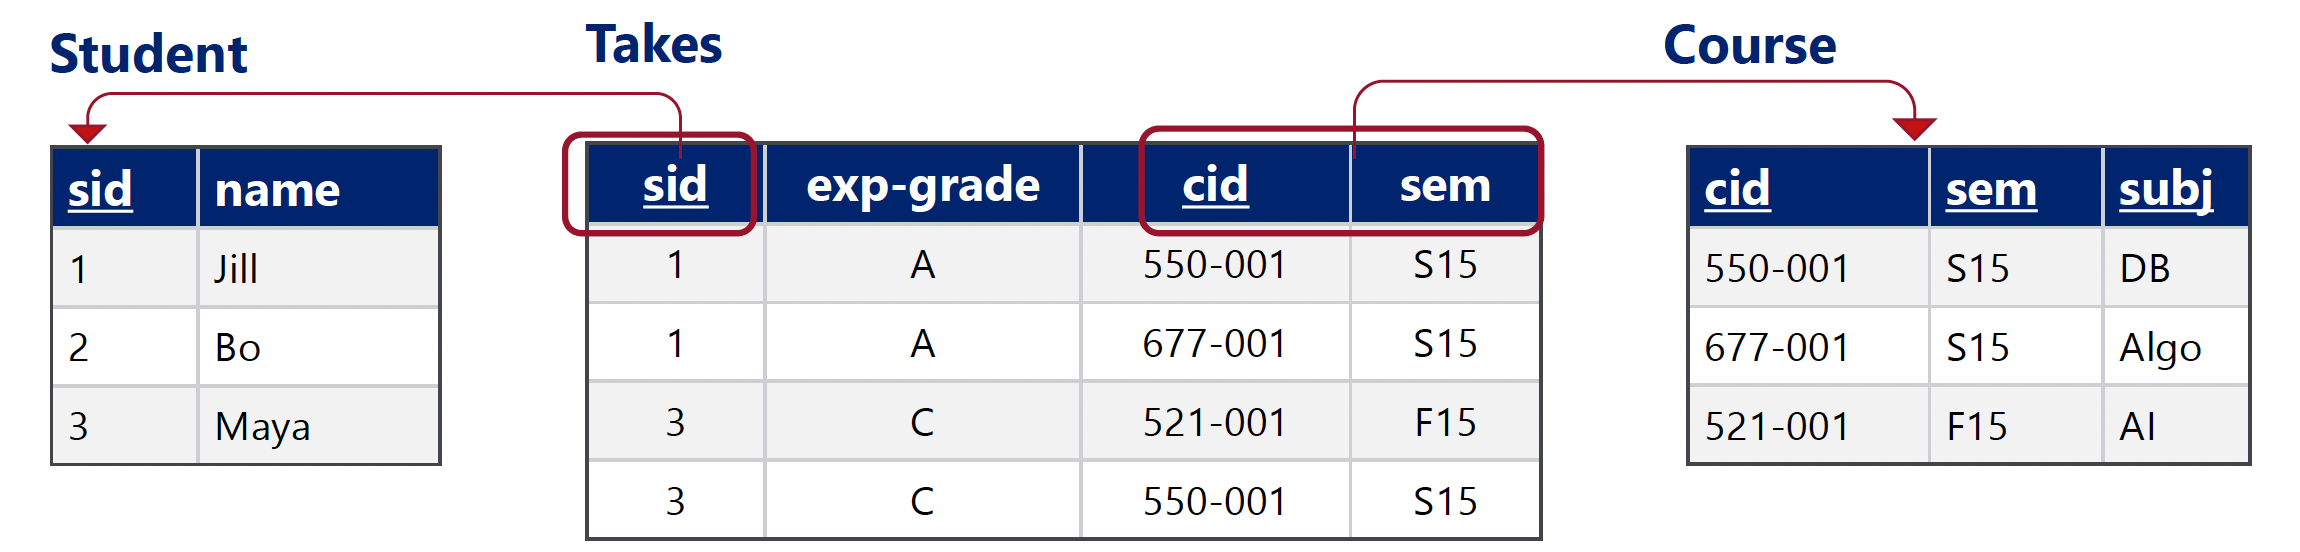
\includegraphics[width=10cm]{Assets/existsExample.png}

Let us now use the above syntax to find all students who have taken a course in DB but not in AI.

\begin{tcolorbox}
    \begin{verbatim}
        SELECT s.sid
        FROM Student s
        WHERE EXISTS 
            (SELECT *
            FROM Takes t JOIN Course c
                ON t.cid = c.cid
            WHERE c.subj = `DB' AND t.sid = s.sid)
        AND NOT EXISTS
            (SELECT *
            FROM Takes t JOIN Course c
                ON t.cid = c.cid
            WHERE c.subj = `AI' AND t.sid = s.sid);
    \end{verbatim}
\end{tcolorbox}

Keep in mind that it really does not matter what we \textit{SELECT} within these subqueries since in either case, the query is just going to be checking to see if there is at least one tuple that meets our conditions at which point it basically returns a boolean -- either \textit{True} or \textit{False}.

\section*{Aggregation}

Aggregation in SQL refers to the use of functions that take multiple rows of input and output a single value. This concept goes well beyond the original proposal by Codd for a relational database since the output of the query may include values not in the database. Aggregation is essential for data analytics and some of these functions are: \textit{MIN}, \textit{MAX}, \textit{COUNT}, and \textit{AVG}.

Here are some examples of the above functions:

\begin{tcolorbox}
    \begin{verbatim}
        SELECT COUNT(*) AS num
        FROM Person

        SELECT AVG(age)
        FROM Person

        SELECT MAX(age)
        FROM Person
    \end{verbatim}
\end{tcolorbox}

Their function should be readily apparent but the first returns the number of tuples in Person, the second returns the average age in Person, and the third returns the oldest age in Person.

Now we further improve our data analysis abilities by use of \textit{GROUP BY} syntax. Here is the general format for using it along with some other related and new syntax:

\begin{tcolorbox}
    \begin{verbatim}
        SELECT {group-attribs}, {aggregate-operator} (attrib),
            ..., {aggregate-operator} (attrib)
        FROM {list of relations}
        WHERE {condition}
        GROUP BY {group-attribs}
        [HAVING {condition on aggregate}]
    \end{verbatim}
\end{tcolorbox}

Keep in mind that we can use the \textit{DISTINCT} keyword for these aggregate operators: \textit{AVG}, \textit{COUNT}, and \textit{SUM}.

Now, let us work through some examples. Here is the relevant relation:

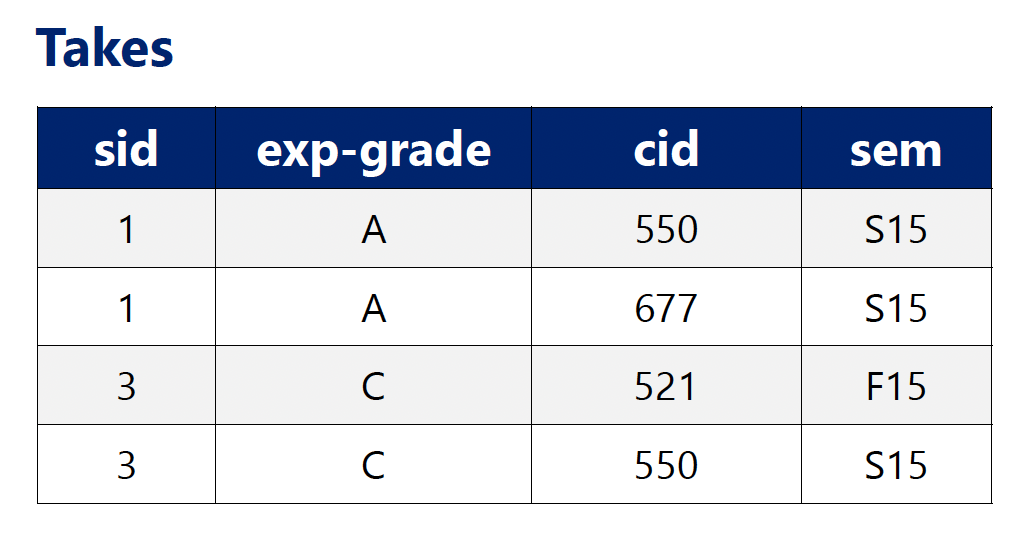
\includegraphics[width=10cm]{Assets/groupByExample.png}

So, what should our query be if we want a relation outputted that has the schema : (\textit{cid}, \textit{sem}, \textit{num}) where \textit{num} is the number of students in each course offering.

\begin{tcolorbox}
    \begin{verbatim}
        SELECT cid, sem, COUNT(*) AS num
        FROM Takes
        GROUP BY cid, sem
    \end{verbatim}
\end{tcolorbox}

Okay, now what if we want the number of different grades expected for each student (Schema: (\textit{sid}, \textit{num}))?

\begin{tcolorbox}
    \begin{verbatim}
        SELECT sid, COUNT(DISTINCT exp-grade) AS num
        FROM Takes
        GROUP BY sid
    \end{verbatim}
\end{tcolorbox}

Then, we can further parse our query output by only outputting tuples that meet some condition which utilizes an aggregate value. This can be done using the \textit{HAVING} clause which we got a glimpse of earlier.

Okay now let's take a look at another relation:

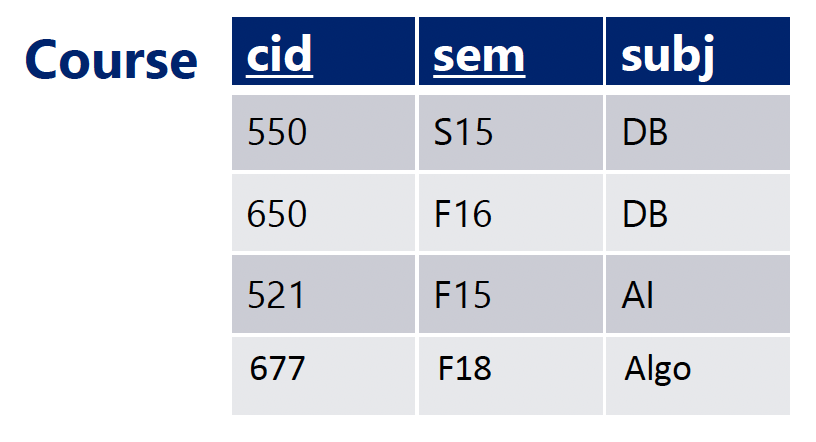
\includegraphics[width=10cm]{Assets/havingExample.png}

Our goal is such: for each subject that is not `AI' which has more than 1 course, print the number of courses. \textit{Schema: (subj, num)}

\begin{tcolorbox}
    \begin{verbatim}
        SELECT subj, COUNT(*) AS num
        FROM Course
        WHERE subj <> `AI'
        GROUP BY subj
        HAVING COUNT(*) > 1
    \end{verbatim}
\end{tcolorbox}

Keep in mind that only grouping attributes, so attributes which we group by, and aggregate operations over attributes can appear in the \textit{SELECT} clause.

\section*{NULL values}

What do we do when we are missing some information? We can use \textbf{NULL} values. Well, how do we evaluate Boolean expressions while accounting for these NULL values? We must use three-state logic where the result of a Boolean expression can be true(T), false(F) or unknown(U).

Pretty easy actually, let's go one by one and keep in mind that we can consider $T = 1$, $F = 0$, $U = 0.5$:
\begin{itemize}
    \item AND
    \begin{itemize}
        \item T AND T = T
        \item Use MIN(X,Y) to calculate Boolean expressions including U and AND
        \begin{itemize}
            \item T AND U = MIN(1,0.5) = U
            \item F AND U = MIN(0, 0.5) = F
            \item U AND U = MIN(0.5, 0.5) = U
        \end{itemize}
    \end{itemize}
    \item OR
    \begin{itemize}
        \item T OR U = T
        \item Use MAX(X,Y) to calculate Boolean expressions including U and OR
        \begin{itemize}
            \item T OR U = MAX(1, 0.5) = T
            \item F OR U = MAX(0, 0.5) = U
            \item U OR U = MAX(0.5, 0.5) = U
        \end{itemize}
    \end{itemize}
    \item NOT
    \begin{itemize}
        \item NOT F = T
        \item Use 1 - X to calculate Boolean expressions including U and NOT
        \begin{itemize}
            \item NOT U = 1 - 0.5 = U
        \end{itemize}
    \end{itemize}
\end{itemize}
\begin{itemize}
    \item Okay, what about if a NULL value is in a comparison? Then, the result is just UNKNOWN (U).
    \item If a NULL value is present in an arithmetic operation, then the result is NULL
    \item NULL values are ignored in an aggregation, except for in COUNT(*) where all tuples are counted, including those containing NULLs

Now, let us consider which tuple bindings are included in query outputs. There is a rule in SQL that only tuple bindings that yield True are included in the output.

We can also directly address the case where we encounter a NULL value by using this syntax:

\begin{tcolorbox}
    \begin{verbatim}
        x is NULL
        x IS NOT NULL
    \end{verbatim}
\end{tcolorbox}
\end{itemize}

In practice, we would get queries that look something like this:
\begin{tcolorbox}
    \begin{verbatim}
        SELECT *
        FROM Person
        WHERE age < 25 OR age >= 25
            OR age IS NULL
    \end{verbatim}
\end{tcolorbox}

Note that when using \textit{JOIN...ON} syntax, you can specify \textit{LEFT OUTER JOIN} or \textit{RIGHT OUTER JOIN} which means you keep all of the records from the relation on the specified side and only matching records from the opposing side. There is also \textit{FULL OUTER JOIN} for when you want to keep all records from both relations. An example of this can be seen below with the corresponding relations:

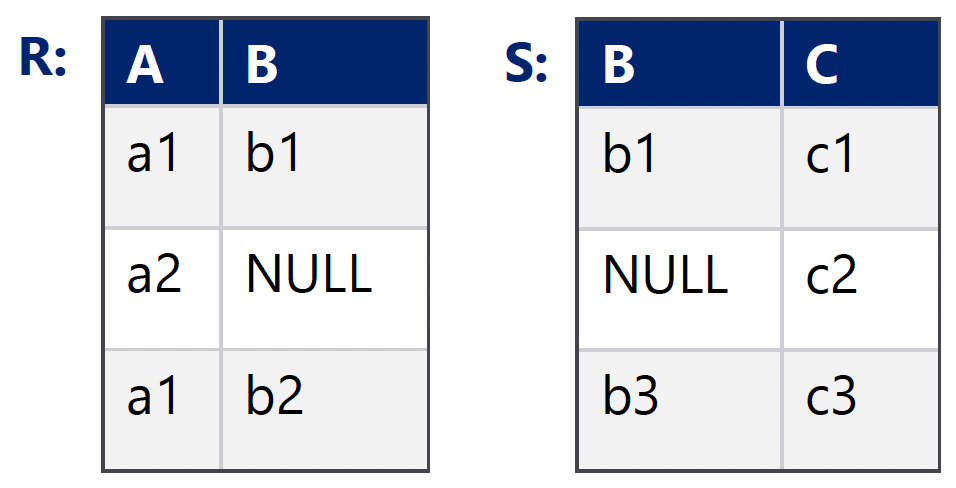
\includegraphics[width=10cm]{Assets/nullJoins.png}

And calling the following query:

\begin{tcolorbox}
    \begin{verbatim}
        SELECT *
        FROM R LEFT OUTER JOIN S ON R.B = S.B
    \end{verbatim}
\end{tcolorbox}

Gives this output:

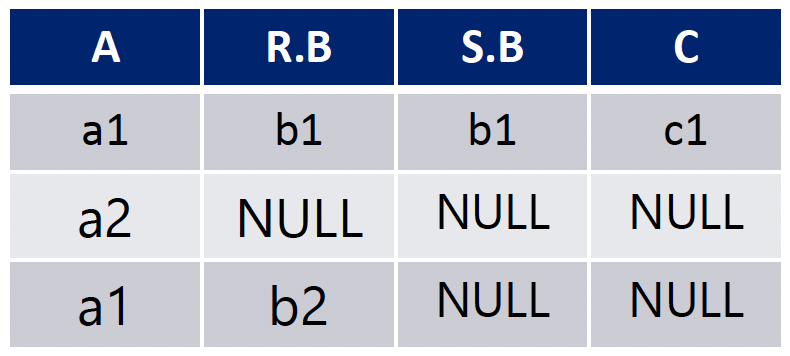
\includegraphics[width=10cm]{Assets/leftOuterJoin.png}

Note that if you use the \textit{DISTINCT} keyword, all NULLs are treated as equal and at most one NULL is outputted. On the other hand, \textit{COUNT (DISTINCT \{attr\})} does not count NULLs.

Further, \textit{GROUP BY} treats all NULLs as equal, so you output at most one group of NULLs which you can then apply any aggregation function to, including \textit{COUNT}.

Moreover, \textit{UNION}, \textit{INTERSECT}, and \textit{EXCEPT} treat all NULLs as equal so you output at most one NULL in the query output. On the other hand: \textit{UNION ALL}, \textit{INTERSECT ALL}, and \textit{EXCEPT ALL} treat all NULLs as distinct so you may output any number of them.

By default, any column can hold NULL values except for primary key columns. While defining a table using SQL DDL(Data Definition Language), we can disallow NULL values in a particular column using the \textit{NOT NULL} syntax. Refer to the example below so you may refresh your memory of SQL DDL.

\begin{tcolorbox}
    \begin{verbatim}
        CREATE TABLE Persons (
            ID int,
            LastName varchar(255) NOT NULL,
            FirstName varchar(255) NOT NULL,
            Age int,
            PRIMARY KEY (ID)
        );
    \end{verbatim}
\end{tcolorbox}

Closing out this section, recall that only bindings in the \textit{FROM} clause that evaluate to True in the \textit{WHERE} clause are returned. Further, keep in mind that NULL in an arithmetic expression evaluates to NULL and that NULL in a comparison evaluates to UNKNOWN.

\section*{Different Flavors of Joins}

Our first new flavor of joins is the \textbf{cross product}! Let's look at an example query that does this:

\begin{tcolorbox}
    \begin{verbatim}
        SELECT *
        FROM Employee, Department
    \end{verbatim}
\end{tcolorbox}

As you can see, we're asking for all tuples from both the relations \textit{Employee} and \textit{Department} in one table. The only reasonable output is for each tuple from \textit{Employee} to merge with every tuple in \textit{Department}. Note that the size of the cross product of two relations in terms of their cardinalities $n_1$ and $n_2$ is $n_1 \cdot n_2$.

Now, we move on to the \textbf{Equijoin}. This is one we've come across quite a bit, especially with matching key-foreign key relationships. We can also use the \textit{JOIN...ON} syntax for non-key attributes. Importantly, equijoins between non-key attributes may have a query output with a cardinality that has the same size as a cross product. And equijoins for key-foreign key relationships, if the key relation has cardinality $n_1$ and the foreign key relation has cardinality $n_2$, have a query output cardinality of $n_2$.

One that is really easy to understand is the \textbf{Natural Join} which just combines columns using column names. An example query can be seen below:

\begin{tcolorbox}
    \begin{verbatim}
        SELECT *
        FROM Employee NATURAL JOIN Department
    \end{verbatim}
\end{tcolorbox}

Keep in mind that a natural join where the two component relations share the same schema is equivalent to querying for which tuples in either relation are exactly the same. And if no column names match across the two relations, then this is a disjoint schema and the natural join just ends up outputting the cross product.

And recall that we've discussed the following types of joins previously:
\begin{itemize}
    \item Left outer join: Include the left tuple even if there's no match
    \item Right outer join: Include the right tuple even if there's no match
    \item Full outer join: Include both the left and right tuples even if there's no match
\end{itemize}

\section*{Updates}
Tuples can be inserted into a database explicitly, or we can just insert the results of a query. Examples of both approaches are listed below:

\begin{tcolorbox}
    \begin{verbatim}
        INSERT INTO professor (fid, name)
        VALUES (4, `Simpson')

        INSERT INTO professor (fid, name)
            SELECT sid AS fid, name
            FROM student
            WHERE sid < 20
    \end{verbatim}
\end{tcolorbox}

Deletion and modification of tuples is also simple, but keep in mind that unless a key is used, more than one tuple may be deleted or modified. Below are examples of both:

\begin{tcolorbox}
    \begin{verbatim}
        DELETE
        FROM student s
        WHERE s.sid < 25

        UPDATE student s
        SET s.sid = 2 + s.sid, s.name = `Boon'
        WHERE s.name = `Bo'
    \end{verbatim}
\end{tcolorbox}

You can also use \textit{ALTER TABLE} to add columns to a table. Some DBMS will also allow columns to be dropped using this syntax. Further, column type can be changed using this syntax. Examples of all three uses can be seen below:

\begin{tcolorbox}
    \begin{verbatim}
        ALTER TABLE student
        ADD gpa real NULL

        ALTER TABLE student
        DROP COLUMN gpa

        ALTER TABLE student
        MODIFY COLUMN gpa decimal
    \end{verbatim}
\end{tcolorbox}

Notice how we used other syntax specific for adding, dropping, and modifying columns. We will not delve into them too much, but notice that their meaning is fairly obvious.

We can also add/drop constraints using the same \textit{ALTER TABLE} syntax. I include examples of both below:

\begin{tcolorbox}
    \begin{verbatim}
        ALTER TABLE student
        ADD CONSTRAINT std_pk PRIMARY KEY (sid)

        ALTER TABLE student
        DROP CONSTRAINT std_pk
    \end{verbatim}
\end{tcolorbox}

Note that \textit{std\_pk} is just the name we give to the constraint, stands for `student primary key'.

We can also use the \textit{DROP} command to delete tables (and temporary tables) and all of their content, as well as views -- which we have not discussed yet. Refer to examples of both below:

\begin{tcolorbox}
    \begin{verbatim}
        DROP TABLE student
        
        DROP VIEW Top_Students
    \end{verbatim}
\end{tcolorbox}

\section*{Views}
A view is a named query that can be used in other queries. An example of a view being created and then used can be seen below:

\begin{tcolorbox}
    \begin{verbatim}
        CREATE VIEW Top_Students (sid, sname, gpa) AS
        SELECT s.sid, s.sname, s.gpa FROM Student
        WHERE s.gpa >= 3.85

        SELECT t.cid
        FROM Top_Students ts, Takes t
        WHERE ts.sid = t.sid
    \end{verbatim}
\end{tcolorbox}

Importantly, unlike a temporary table, a view is computed upon request and is therefore always up-to-date. And unlike a Common Table Expression (CTE), the view persists until it is dropped.

Views are useful because they can simplify complex queries, they can facilitate security/access control by having different user groups seeing different views of the database. Views can also be used in query optimization -- so if materialized, i.e. stored and updated as the database changes. Views can also be used to describe transformations or mappings from one schema to another.

Going back to materialized views, they are computed once and stored statically. But they must be updated as the underlying database changes. These updates can occur either manually or be made to occur periodically.

If a view can be updated, then the update propagates to the base relations. However, there are a lot of views which are not updatable. Here is how to tell if a view is updatable: the view is defined on a single base table (multiple source relations would really complicate updates), it uses only selection and projection (only simple operations where projection means choosing which columns are returned by the query and selection means choosing which rows are returned by the query), there are no aggregates (unclear how an aggregate would update a base relation after all), and \textit{DISTINCT} is not used (merges multiple rows from the base relation so it would be unclear how the base relation would be updated).
\end{document}

